\documentclass[a4paper,12pt]{article}

%%% Работа с русским языком
\usepackage{cmap}					% поиск в PDF
\usepackage{mathtext} 				% русские буквы в формулах
\usepackage[T2A]{fontenc}			% кодировка
\usepackage[utf8]{inputenc}			% кодировка исходного текста
\usepackage[english,russian]{babel}	% локализация и переносы
\usepackage{xcolor}
\usepackage{hyperref}
 % Цвета для гиперссылок
\definecolor{linkcolor}{HTML}{799B03} % цвет ссылок
\definecolor{urlcolor}{HTML}{799B03} % цвет гиперссылок

\hypersetup{pdfstartview=FitH,  linkcolor=linkcolor,urlcolor=urlcolor, colorlinks=true}

%%% Дополнительная работа с математикой
\usepackage{amsfonts,amssymb,amsthm,mathtools} % AMS
\usepackage{amsmath}
\usepackage{icomma} % "Умная" запятая: $0,2$ --- число, $0, 2$ --- перечисление

%% Номера формул
%\mathtoolsset{showonlyrefs=true} % Показывать номера только у тех формул, на которые есть \eqref{} в тексте.

%% Шрифты
\usepackage{euscript}	 % Шрифт Евклид
\usepackage{mathrsfs} % Красивый матшрифт

%% Свои команды
\DeclareMathOperator{\sgn}{\mathop{sgn}}

%% Перенос знаков в формулах (по Львовскому)
\newcommand*{\hm}[1]{#1\nobreak\discretionary{}
{\hbox{$\mathsurround=0pt #1$}}{}}
% графика
\usepackage{graphicx}
\graphicspath{{pictures/}}
\DeclareGraphicsExtensions{.pdf,.png,.jpg}
\author{Бурмашев Григорий, БПМИ-208}
\title{}
\date{\today}
\begin{document}
\begin{center}
Бурмашев Григорий. ИДЗ -- 6.
\end{center}
\section*{Номер 1}
\[
Q(x_1, x_2, x_3) = -1x_1^2 + 21x_2^2 - 60x_3^2 - 4x_1x_2 + 18x_1x_3 + 86x_2x_3
\]
\begin{enumerate}
\item
Воспользуемся методом Лагранжа, чтобы найти нормальный вид:
\[
-(x_1 + 2x_2 - 9x_3)^2 + 4x_2^2 + 81x_3^2 - 36x_2x_3 + 21x_2^2 - 60x_3^2 + 86x_2x_3 = 
\]
\[
=
-(x_1 + 2x_2 - 9x_3)^2  + 25x_2^2 + 21x_3^2 + 50x_2x_3 = 
\]
\[
=
-(x_1 + 2x_2 - 9x_3)^2 + (5x_2 + 5x_3)^2 + 21x_3^2 - 25x_3^2 = -(x_1 + 2x_2 - 9x_3)^2 + (5x_2 + 5x_3)^2 - 4x_3^2
\]
Введем замену координат:
\[
\widetilde{x_1} = x_1 + 2x_2 - 9x_3
\]
\[
\widetilde{x_2} = 5x_2 + 5x_3
\]
\[
\widetilde{x_3} = 2x_3
\]
Тогда получаем:
\[
Q(x_1, x_2,x_3) = - \widetilde{x_1}^2 + \widetilde{x_2}^2 - \widetilde{x_3}^2
\]
\item
Найдем выражение старых координат через новые. Для этого введем матрицу замены базиса C. Тогда мы знаем матрицу $C^{-1}$ (из $x_i$ в $\widetilde{x_i}$):
\[
C^{-1}= 
\begin{pmatrix}
1 & 2 & -9 \\
0 & 5 & 5 \\
0 & 0 & 2
\end{pmatrix}
\]
Тогда найдем $C$:
\[
\begin{pmatrix}
1 & 2 & -9 & \vrule &1 & 0 & 0  \\
0 & 5 & 5  & \vrule &0 & 1 & 0  \\
0 & 0 & 2 & \vrule &0 & 0 & 1  \\
\end{pmatrix}
=
\begin{pmatrix}
1 & 2 & -9 & \vrule &  1 & 0 & 0 \\
0 & 1 & 1 & \vrule & 0 & \frac{1}{5} & 0 \\
0 & 0 & 1 & \vrule & 0 & 0 & \frac{1}{2} \\
\end{pmatrix}
=
\]
\[
=
\begin{pmatrix}
1 & 2 & -9 & \vrule &  1 & 0 & 0 \\
0 & 1 & 0 & \vrule & 0 & \frac{1}{5} & -\frac{1}{2} \\
0 & 0 & 1 & \vrule & 0 & 0 & \frac{1}{2} \\
\end{pmatrix}
=
\begin{pmatrix}
1 & 0 & 0 & \vrule &  1 &-\frac{2}{5} & \frac{11}{2} \\
0 & 1 & 0 & \vrule & 0 & \frac{1}{5} & -\frac{1}{2} \\
0 & 0 & 1 & \vrule & 0 & 0 & \frac{1}{2} \\
\end{pmatrix}
\]
Тогда:
\[
C
=
\begin{pmatrix}
 1 &-\frac{2}{5} & \frac{11}{2} \\
0 & \frac{1}{5} & -\frac{1}{2} \\
 0 & 0 & \frac{1}{2} \\
\end{pmatrix}
\]
Отсюда выражение координат:
\[
x_1 = \widetilde{x_1} - \frac{2}{5} \widetilde{x_2}  + \frac{11}{2} \widetilde{x_3}
\]
\[
x_2 = \frac{1}{5} \widetilde{x_2} - \frac{1}{2} \widetilde{x_3}
\]
\[
x_3 = \frac{1}{2} \widetilde{x_3}
\]
\end{enumerate}
\begin{center}
\textbf{Ответ: } 

нормальный вид:
\[
Q(x_1, x_2, x_3) = - \widetilde{x_1}^2 + \widetilde{x_2}^2 - \widetilde{x_3}^2
\]
выражение старых координат через новые:
\[
x_1 = \widetilde{x_1} - \frac{2}{5} \widetilde{x_2}  - \frac{11}{4} \widetilde{x_3}
\]
\[
x_2 = \frac{1}{5} \widetilde{x_2} + \frac{1}{4} \widetilde{x_3}
\]
\[
x_3 = \frac{1}{2} \widetilde{x_3}
\]
\end{center}
\clearpage
\section*{Номер 2}
\[
Q(x_1, x_2, x_3) = 6x_1^2 + (6b+2)x_2^2 + (6b-1)x_3^2 + 2x_1x_2 - 8x_1x_3 + 2(6b+5)x_2x_3
\]
Матрица квадратичной формы:
\[
\begin{pmatrix}
6 & 1 & -4 \\
1 & 6b + 2& 6b + 5 \\
-4 & 6b + 5  & 6b - 1 \\
\end{pmatrix}
\]
Найдем угловые миноры этой матрицы:
\begin{enumerate}
\item
$\triangle_1 = 6$
\item
$\triangle_2 = 6(6b+2) -1 = 36b + 11$
\item
$\triangle_3 = 6(6b+2)(6b-1) + (6b+5)(-4) -4(6b+5) +4(6b+2)(-4) - (6b+5)(6b+5)6 - (6b-1) = -474b - 233 $
Приравняем $\triangle_2$ и $\triangle_3$ к нулю, чтобы найти точки b:
\[
36b + 11 = 0; b = -\frac{11}{36}
\]
\[
-474b - 233 = 0; b = -\frac{233}{474}
\]
\end{enumerate}
\begin{center}
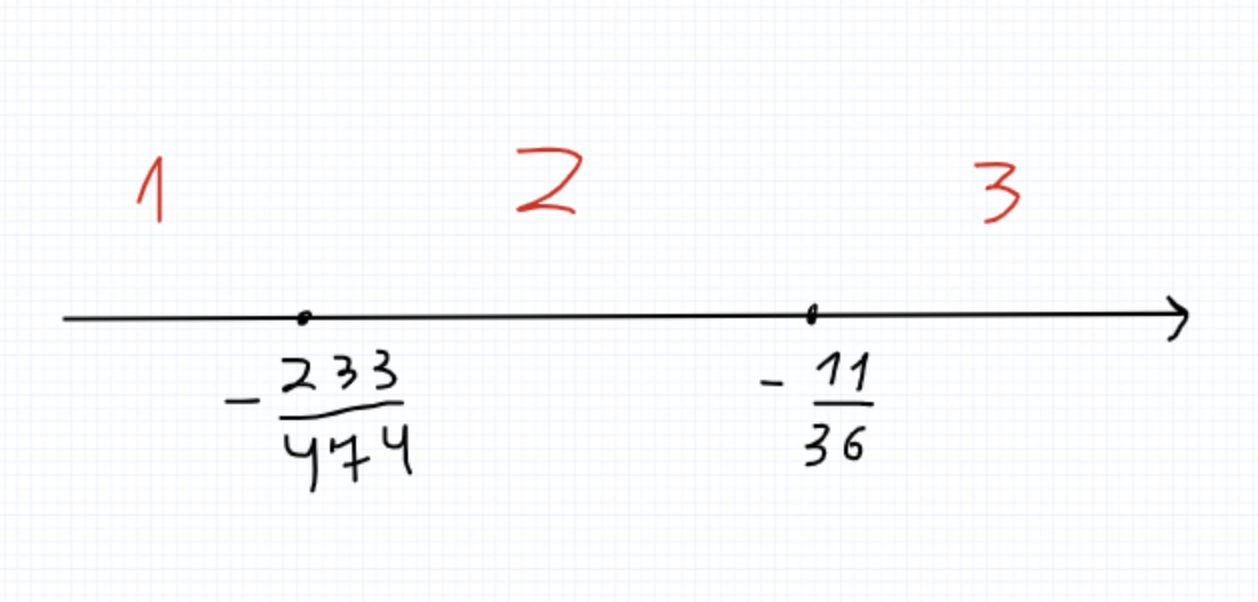
\includegraphics[scale=0.4]{1.png}
\end{center}
Посмотрим на сигнатуры на всех участках:
\begin{enumerate}
\item  $\triangle_1 > 0, \triangle_2 < 0, \triangle_3 < 0$ : $++-$ (1 перемена знаков)
\item  $\triangle_1 > 0, \triangle_2 < 0, \triangle_3 > 0$ : $+--$ (2 перемены знаков)
\item $\triangle_1 > 0, \triangle_2 > 0, \triangle_3 > 0$ :  $+++$ (знаки не меняются)
\end{enumerate}
Отдельно посмотрим на случаи, когда $\triangle_2$ и $\triangle_3$ равны нулю:
\begin{itemize}
\item $b = -\frac{233}{474}$: 
\[
\triangle_1 > 0,  \triangle_2 < 0, \triangle_3 = 0 : +- \text{ (1 перемена знака)}
\]
\item $b = -\frac{11}{36}$:
\end{itemize}
Тут мы уже не можем приравнять $\triangle_2$ к нулю, ибо он является промежуточным, нам нужно заменять координаты, чтобы понять сигнатуру: 
\[
Q(x_1, x_2, x_3) = 6x_1^2 + (6b+2)x_2^2 + (6b-1)x_3^2 + 2x_1x_2 - 8x_1x_3 + 2(6b+5)x_2x_3
\]
Введем замену координат:
\[
\widetilde{x_1} = x_3
\]
\[
\widetilde{x_2} = x_2
\]
\[
\widetilde{x_3} = x_1
\]
Тогда:
\[
Q(x_1,x_2, x_3) = 6\widetilde{x_3} ^2 + (6b+2)\widetilde{x_2} ^2 + (6b-1)\widetilde{x_1} ^2 + 2\widetilde{x_3} \widetilde{x_2}  - 8\widetilde{x_3}\widetilde{x_1}  + 2(6b+5)\widetilde{x_2} \widetilde{x_1} 
\]
Отсюда матрица квадратичной формы в новых координатах:
\[
\begin{pmatrix}
6b-1 & 6b+5& -4 \\
6b+5 & 6b+2 & 1 \\
-4 & 1 & 6 \\
\end{pmatrix}
\]
Подставляем $b = -\frac{11}{36}$:
\[
\begin{pmatrix}
-\frac{17}{6} & \frac{19}{6}& -4 \\ 
\frac{19}{6} & \frac{1}{6}& 1 \\
-4 & 1 & 6 \\
\end{pmatrix}
\]
Тогда угловые миноры будут равны:
\[
\triangle_1 = -\frac{17}{6} < 0
\]
\[
\triangle_2 = -\frac{17}{6} \cdot \frac{1}{6} - \frac{19}{6} \cdot \frac{19}{6}  = -\frac{21}{2} < 0 
\]
\[
\triangle_3 = -\frac{529}{6} < 0 
\]
Перемен знаков нет, значит сигнатура $+++$
\clearpage
\begin{center}
\textbf{Ответ: } 
\begin{itemize}
\item
$b < \frac{233}{474}$:
\[
\widetilde{x_1}^2 + \widetilde{x_2}^2  - \widetilde{x_3}^2 
\]
\item
$b \in (-\frac{233}{474}; -\frac{11}{36})$:
\[
\widetilde{x_1}^2  - \widetilde{x_2}^2  - \widetilde{x_3}^2 
\]
\item
$b > -\frac{11}{36}:$
\[
\widetilde{x_1}^2  + \widetilde{x_2}^2  + \widetilde{x_3}^2 
\]
\item
$b = -\frac{233}{474}:$
\[
\widetilde{x_1}^2  - \widetilde{x_2}^2 
\]
\item
$ b = - \frac{11}{36}$:
\[
\widetilde{x_1}^2  +\widetilde{x_2}^2 +\widetilde{x_3}^2 
\]
\end{itemize}
\end{center}
\clearpage
\section*{Номер 3}
\[
\beta (x, y) = (-4b + 17) x_1y_1 + (-2b+8)x_1y_2 + (-2b+7)x_1y_3 +
\]
\[
+
 (-2b+8)x_2y_1 + 2x_2y_2 + (-2b+6)x_2y_3 + (-a + 3.5)x_3y_1  + (-2b + b) x_3y_2 + 3x_3y_3
\]
Нам нужно, чтобы биллинейная форма была симметричной, а также ее квадратичная форма была положительно определена.
\begin{enumerate}
\item
Проверим симметричность, для этого посмотрим на матрицу биллинейной формы:
\[
\begin{pmatrix}
-4b + 17 & -2b + 8 & -2b + 7\\
-2b + 8 & 2& -2b + 6 \\
-a + 3.5 & -2b + 6 &3 \\
\end{pmatrix}
\]
Для симметрии нужно, чтобы $-a + 3.5 = -2b + 7$, а значит получаем точное значение для а:
\[
a = 2b - 3.5
\]
Тогда матрица:
\[
\begin{pmatrix}
-4b + 17 & -2b + 8 & -2b + 7\\
-2b + 8 & 2& -2b + 6 \\
-(2b-3.5) + 3.5 & -2b + 6 &3 \\
\end{pmatrix}
\]
\item Теперь найдем, найдем угловые миноры и воспользуемся критерием Сильвестра (угловые миноры должны быть больше нуля):
\[
\triangle_1 = -4b + 17;
\]
Отсюда $b < \frac{17}{4} = 4.25$
\[
\triangle_2 = (-4b+17) \cdot 2 - (-2b+8) \cdot (-2b+8) = -4b^2 + 24b - 30
\]
Отсюда $b \in \left( \frac{6 - \sqrt{6}}{2}; \frac{6 + \sqrt{6}}{2}\right)$
\[
\triangle_3 = (-4b+17) \cdot 6 + (-2b+8)(-2b+6)(-2b+7) + (-2b+7)(-2b+8)(-2b+6) -
\]
\[
-
 (-2b+7) \cdot 2 \cdot(-2b+7) - (-2b+6)(-2b+6)(-4b+17) -3(-2b+8)(-2b+8) = 
\]
\[
 = -16b^2 + 96b -128
\]
Отсюда $b \in (2, 4)$

Самое строгое условие у нас у $\triangle_3$, значит, чтобы все миноры были больше нуля, нужно, чтобы $b \in (2, 4)$.

Тогда, поскольку $a = 2b -3.5$, то $a \in (0.5;  4.5)$
\end{enumerate}
\section*{Номер 4}
Матрица:
\[
\begin{pmatrix}
33 & -21 & -48 \\
-21 & 18 & 12 \\
-48 & 12 & 144
\end{pmatrix}
\]
Посчитаем угловые миноры матрицы Грама:
\[
\triangle_1 = 33 \\
\]
\[
\triangle_2 = 33 \cdot 18 - 21 \cdot (-21) = 153
\]
\[
\triangle_3 =  33 \cdot 18 \cdot 144 -21 \cdot 12 \cdot (-48) + 48 \cdot 21 \cdot 12 +  
\]
\[
+
48 \cdot 18 \cdot (-48) - 12 \cdot 12 \cdot 33 - 144 \cdot (-21) \cdot (-21) = 0 
\]
Они все $\geq 0 $, к тому же определитель матрицы равен нулю, а значит мы сможем найти систему векторов, матрица Грама которой будет равна заданной матрице.

Запишем в виде квадратичной формы $Q(x_1, x_2, x_3)$ и соотвественно приведем к стандартному виду методом Лагранжа:
\[
Q(x_1, x_2, x_3) = 33x_1^2 + 18x_2^2 + 144x_3^2 - 42x_1x_2 -96x_1x_3 + 24x_2x_3 =
\]
\[
33(x_1 - \frac{21}{33}x_2 - \frac{48}{33}x_3)^2 + 18x_2^2 + 144x_3^2 +24x_2x_3 + \frac{441}{33}x_2^2 + \frac{2304}{33} x_3^2 + \frac{2016}{33} x_2x_3 = 
\]
\[
= 33\left(x_1 - \frac{7}{11}x_2 - \frac{16}{11}x_3\right)^2 + 18x_2^2 + 144x_3^2 + 24x_2x_3 - \frac{147}{11}x_2^2 - \frac{768}{11}x_3^2 - \frac{672}{11}x_2x_3 =
\]
\[
= 33\left(x_1 - \frac{7}{11}x_2 - \frac{16}{11}x_3\right)^2 + \frac{51}{11}x_2^2 + \frac{816}{11}x_3^2 - \frac{408}{11}x_2x_3 = 
\]
\[
=
33\left(x_1 - \frac{7}{11}x_2 - \frac{16}{11}x_3\right)^2 + \frac{51}{11}(x_2 - 4x_3)^2 + \frac{408}{11}x_2x_3 - \frac{408}{11}x_2x_3 = 
\]
\[
=
33\left(x_1 - \frac{7}{11}x_2 - \frac{16}{11}x_3\right)^2 + \frac{51}{11}(x_2 - 4x_3)^2 
\]
Введем замену координат:
\[
\widetilde{x_1} = x_1 - \frac{7}{11}x_2- \frac{16}{11}x_3
\]
\[
\widetilde{x_2} = x_2 - 4x_3
\]
\[
\widetilde{x_3} = x_3
\]
Тогда в новых координатах матрица квадратичной формы будет:
\[
D = 
\begin{pmatrix}
33 & 0 & 0 \\
0 & \frac{51}{11} & 0 \\
0 & 0 & 0 \\
\end{pmatrix}
\]
А матрица $D'$ (корни от каждого элемента матрицы) :
\[
\begin{pmatrix}
\sqrt{33}& 0 & 0 \\
0 & \sqrt{\frac{51}{11}}& 0 \\
0 & 0 & 0 \\
\end{pmatrix}
\]
А матрица перехода от новых координат к старым ($C^{-1}$)
\[
C^{-1} = 
\begin{pmatrix}
1 & -\frac{7}{11} &  -\frac{16}{11} \\
0 & 1 & -4 \\
0 & 0 & 1 \\
\end{pmatrix}
\]
Тогда искомые три вектора будут находиться в столбцах матрицы $D' \cdot C^{-1}$:
\[
D' \cdot C^{-1} = 
\begin{pmatrix}
\sqrt{33}& 0 & 0 \\
0 & \sqrt{\frac{51}{11}}& 0 \\
0 & 0 & 0 \\
\end{pmatrix}
\cdot
\begin{pmatrix}
1 & -\frac{7}{11} &  -\frac{16}{11} \\
0 & 1 & -4 \\
0 & 0 & 1 \\
\end{pmatrix}
=
\left(\begin{matrix}
\sqrt{33} & \frac{-7\sqrt{33}}{11} & \frac{-16\sqrt{33}}{11} \\
0 & \frac{\sqrt{561}}{11} & \frac{-4\sqrt{561}}{11} \\
0 & 0 & 0
\end{matrix}\right)
\]
По итогу (наконец-то) получаем векторы:
\[
\begin{pmatrix}
\sqrt{33} \\ 0 \\ 0
\end{pmatrix}
;
\begin{pmatrix}
 \frac{-7\sqrt{33}}{11} \\ \frac{\sqrt{561}}{11} \\ 0 
\end{pmatrix}
;
\begin{pmatrix}
\frac{-16\sqrt{33}}{11}  
\\
\frac{-4\sqrt{561}}{11}
\\
0
\end{pmatrix}
\]
\clearpage
\begin{center}
\textbf{Ответ: } 
\[
\begin{pmatrix}
\sqrt{33} \\ 0 \\ 0
\end{pmatrix}
;
\begin{pmatrix}
 \frac{-7\sqrt{33}}{11} \\ \frac{\sqrt{561}}{11} \\ 0 
\end{pmatrix}
;
\begin{pmatrix}
\frac{-16\sqrt{33}}{11}  
\\
\frac{-4\sqrt{561}}{11}
\\
0
\end{pmatrix}
\]
\end{center}
\end{document}
